\documentclass[a4paper,12pt,russian]{extreport}

\usepackage{extsizes}
\usepackage{titlesec}
\usepackage{cmap}
\usepackage[T2A]{fontenc}
\usepackage[utf8]{inputenc}
\usepackage[russian]{babel}

%\usepackage{pscyr}
\usepackage{graphicx}
\usepackage{amsmath, amsthm, amsfonts}
\usepackage{indentfirst}
\usepackage[usenames,dvipsnames]{color}
\usepackage[table,xcdraw]{xcolor}
\usepackage{makecell}
\usepackage{multirow}
\usepackage{ulem}
\usepackage{tocloft}
\usepackage{import}
\usepackage{lastpage}
\usepackage{etoolbox}
\usepackage[title,titletoc]{appendix}
\usepackage{pdfpages}
\usepackage{listings}
\usepackage{todonotes}
\usepackage{xr}
\usepackage{dsfont}
\usepackage{algorithm2e}

\usepackage[font=it]{caption}
\usepackage{fancyhdr}
\pagestyle{fancy}
\fancyhf{}
\fancyhead[R]{\thepage}
\fancyheadoffset{0mm}
\fancyfootoffset{0mm}
\setlength{\headheight}{17pt}
\renewcommand{\headrulewidth}{0pt}
\renewcommand{\footrulewidth}{0pt}
\fancypagestyle{plain}{
	\fancyhf{}
	\rhead{\thepage}}
\setcounter{page}{5}

\linespread{1.3}
% \renewcommand{\rmdefault}{ftm}
\frenchspacing

\titleformat{\chapter}[display]
	{\filcenter}
	{\MakeUppercase{\chaptertitlename} \thechapter}
	{8pt}
	{\bfseries}{}
	
\titleformat{\paragraph}[display]
	{\filcenter}
	{\MakeUppercase{\chaptertitlename} \thechapter}
	{8pt}
	{\bfseries}{}
	
\titleformat{\section}
	{\normalsize\bfseries}
	{\thesection}
	{1em}{}
	
\titleformat{\subsection}
	{\normalsize\bfseries}
	{\thesubsection}
	{1em}{}
	
\titlespacing*{\chapter}{0pt}{-30pt}{8pt}
\titlespacing*{\paragraph}{0pt}{-30pt}{8pt}
\titlespacing*{\section}{\parindent}{*4}{*4}
\titlespacing*{\subsection}{\parindent}{*4}{*4}

\renewcommand{\cfttoctitlefont}{\hspace{0.38\textwidth} \bfseries\MakeUppercase}
\renewcommand{\cftbeforetoctitleskip}{-1em}
\renewcommand{\cftaftertoctitle}{\mbox{}\hfill \\ \mbox{}\hfill{\footnotesize Стр.}\vspace{-2.5em}}
\renewcommand{\cftchapfont}{\normalsize\bfseries \MakeUppercase{\chaptername} }
\renewcommand{\cftsecfont}{\hspace{31pt}}
\renewcommand{\cftsubsecfont}{\hspace{11pt}}
\renewcommand{\cftbeforechapskip}{1em}
\renewcommand{\cftparskip}{-1mm}
\renewcommand{\cftdotsep}{1}
\setcounter{tocdepth}{2}
\setcounter{secnumdepth}{5}

\usepackage[square,numbers]{natbib}
\newcounter{totfigures}
\newcounter{tottables}
\newcounter{totreferences}
\makeatletter
\renewcommand{\@dotsep}{2}
\newcommand{\l@likechapter}[2]{{\bfseries\@dottedtocline{0}{0pt}{0pt}{#1}{#2}}}
\AtEndDocument{%
  \addtocounter{totfigures}{\value{figure}}%
  \addtocounter{tottables}{\value{table}}%
  \immediate\write\@mainaux{%
    \string\gdef\string\totfig{\number\value{totfigures}}%
    \string\gdef\string\tottab{\number\value{tottables}}%
    \string\gdef\string\totref{\number\value{totreferences}}%
  }%
}
\makeatother
\pretocmd{\chapter}{\addtocounter{totfigures}{\value{figure}}}{}{}
\pretocmd{\chapter}{\addtocounter{tottables}{\value{table}}}{}{}
\pretocmd{\bibitem}{\addtocounter{totreferences}{1}}{}{}
\newcommand{\likechapterheading}[1]{
	\begin{center}
	\textbf{\MakeUppercase{#1}}
	\end{center}
	\empline}
\newcommand{\likechapter}[1]{	
	\phantomsection
	\likechapterheading{#1}	
	\addcontentsline{toc}{likechapter}{\texorpdfstring{\MakeUppercase{#1}}{#1}}}
\newcommand{\empline}{\mbox{}\newline}
\renewcommand{\bibnumfmt}[1]{[#1]\hfill}
\renewcommand{\bibsection}{\likechapter{Список литературы}}
\setlength{\bibsep}{0pt}

\newcommand{\append}[1]{
	\clearpage
	\stepcounter{chapter}	
	\paragraph{\MakeUppercase{#1}}
	\empline
	\addcontentsline{toc}{likechapter}{\texorpdfstring{\chaptertitlename~\Asbuk{chapter}\;#1}}{\chaptertitlename~\Asbuk{chapter}:~#1}}
	
\usepackage{geometry}
\geometry{left=3cm}
\geometry{right=1.5cm}
\geometry{top=2.4cm}
\geometry{bottom=2.4cm}

% \usepackage{enumitem}
% \makeatletter
% \AddEnumerateCounter{\asbuk}{\@asbuk}{м)}
% \makeatother
% \setlist{nolistsep}
% \renewcommand{\labelitemi}{-}
% \renewcommand{\labelenumi}{\asbuk{enumi})}
% \renewcommand{\labelenumii}{\arabic{enumii})}


\usepackage[ruled,vlined]{algorithm2e}
\SetKwHangingKw{KwData}{Вход$\rightarrow$} 
\SetKwHangingKw{KwResult}{Выход$\rightarrow$} 

\usepackage[pdftex,bookmarks=true,colorlinks=true,linkcolor=blue,citecolor=Green,linktoc=none]{hyperref}
\newcommand{\term}[1]{\textit{#1}}
\newcommand{\bydef}{\ensuremath{\stackrel{\text{\upshape df}}{=}}}
\newcommand{\<}{\langle}
\renewcommand{\>}{\rangle}
\newcommand{\includechapter}[1]{\subimport{chapter_#1/}{chapter_#1}}
\newcommand{\inputintro}{\input{sec_Intro} \newpage}

\newtheorem{theorem}{Теорема}
\newtheoremstyle{break}
  {\topsep}{\topsep}%
  {\itshape}{}%
  {\bfseries}{}%
  {\newline}{}%
\theoremstyle{break}
% \renewtheorem{proof}{Доказательство}
\newtheorem{definition}{Определение}
\newtheorem{corollary*}{Следствие}
\newtheorem{lemma}{Лемма}
% \newtheorem{example}{Пример}
% \newtheorem*{example-star}{Пример}

% \theoremstyle{remark}
% \newtheorem*{remark}{Замечание}

\newcommand{\setR}{\mathbb{R}}
\newcommand{\setN}{\mathbb{N}}
\newcommand{\setRn}{\mathbb{R}^n}
\newcommand{\setN}{\mathbb{N}}
\newcommand{\manX}{\mathcal{X}}
\newcommand{\bp}{{\bf P}}
\newcommand{\bs}{{\bf s}}
\newcommand{\bw}{{\bf W}}
\newcommand{\bx}{{\bf X}}
\newcommand{\bc}{{\bf C}}
\newcommand{\bd}{{\bf D}}
\newcommand{\bsm}{{\bf s}}
\newcommand{\bl}{{\bf L}}
\newcommand{\by}{{\bf Y}}
\newcommand{\ba}{{\bf A}}
\newcommand{\manM}{\mathcal{M}}
\newcommand{\manH}{\mathcal{H}}
\newcommand{\spn}{S^+(n,p)}

\newcommand{\condset}[2]{\braces{\, #1 \mid #2 \,}}
\newcommand{\walls}[1]{\left | #1 \right |} 
\newcommand{\norm}[2]{\left{||}#1\right{||}_{#2}} 
\newcommand{\set}[1]{\left\{ #1 \right\}}
\newcommand{\inprod}[3]{\left < #1,#2\right >_#3}


\newcommand{\HRule}{\rule{\linewidth}{0.5mm}}

\begin{document}
\begin{titlepage}
\begin{center}

\small Министерство образования и науки Российской Федерации\\[0.7cm]

\small Федеральное государственное автономное образовательное учреждение \\ высшего профессионального образования \\ «Московский физико-технический институт \\ (государственный университет)»\\[0.6cm]

Факультет управления и прикладной математики\\[0.2cm] 
\small Кафедра проблем передачи информации и анализа данных\\[1.2cm]

% Title
% \HRule \\[0.4cm]
{\Large Применение геометрии многообразия симметричных положительно полуопределенных матриц в анализе данных головного мозга\\[0.4cm] }

% \HRule \\[1.5cm]

Выпускная квалификационная работа \\ (магистерская работа)\\[1.0cm]
Направление подготовки: 03.04.01  Прикладные математика и физика\\[1.5cm]

% Author and supervisor
\begin{minipage}[t]{1.0\textwidth}

\begin{flushleft}
Выполнила \\
Студентка гр. 177
\end{flushleft}
\begin{flushright}
Беляева Дарья Геннадиевна \\
\noindent\hrule
\end{flushright}

\begin{flushleft}
Научный руководитель:
\end{flushleft}
\begin{flushright}
Бурнаев Евгений Владимирович, к.ф.-м.н.\\
\noindent\hrule
\end{flushright}

\end{minipage}

\vfill

% Bottom of the page
{\small Москва 2017}

\end{center}
\end{titlepage}

%\newpage\renewcommand{\abstractname}{Аннотация}

\begin{abstract}

\end{abstract}

\newpage\tableofcontents
\newpage\chapter{Введение}
\indent Современные методы неизвазивного исследования мозга, такие как магнитно-резонансная томография (МРТ), в частности, диффузионно-взвешенная МРТ (дМРТ) позволяют отслеживать на макро-уровне связи между различными зонами мозга, позволяя проводить анализ сттруктурного устройства мозга. На основе дМРТ снимков возможно построить карту структурных связей между зонами мозга, представляя его таким образом в виде графа. Аналогично, с помощью функциональной МРТ (фМРТ) возможно построить граф функциональных связей между различными регионами мозга (коннектом). В этой структуре вершины графа предствляют отдельные регионы мозга, а ребра – связи между регионами. Использование коннектомов приобрело большую популярность в нейронауках из предположения, что структура связей позволяет получить понимание особенностей данной модели мозга и определить механизмы его функционирования. \\
\indent Однако диагностика психиатрических и нейродегенеративных заболеваний при помощи МРТ на сегодняшний день не является точной. Другой проблемой является малое количество данных, не позволяющее оценить обобщающую способность алгоритмов, построенных на использовании данных МРТ. \\
\indent С практической точки зрения представляет интерес задача классификации снимков МРТ, позволяющая, к примеру, автоматически определять структурные повреждения мозга, сопутствующие ранней стадии развития нейродегенеративных заболеваний. Для алгоритмов машинного обучения также является важной особенность обработки исходных снимков МРТ и построения коннектомов, поскольку на основе одного снимка возможно получить несколько разных графов в зависимости от алгоритма трактографии, используемого для преобразования. \\
В данной работе рассматривается четыре алгоритма классификации коннектомов, два из которых являются известными, например, алгоритм предложенный в \cite{dodero2015kernel}. Два других алгоритма предложены в этой работе. \\ 
\indent Ключевой особенностью этой работы является рассмотрение пространства симметричных положительно полуопределенных (СППО) и симметричных положительно определенных (СПО) матриц. Риманова геометрия предоставляет сильные инструменты для обработки структурированных данных, представленных в виде СПО матриц. СПО матрицы образуют дифференцируемое многообразие с соответствующей нелинейной структурой. Инструменты римановой геометрии позволяют находить геодезические и их длины для использования в алгоритмах, основанных на вычислении расстояний между объектами данных. В качестве другого подхода к классификации СПО матриц используется проецирование данных на касательное пространство, аппроксимирующее локальную структуру многообразия. Поскольку проекция является линейным преобразованием, спроецированные данные могут быть рассмотрены как обычные векторы.\\
\indent В последние годы инструменты римановой геометрии нашли широкое применение в анализе медицинских данных, в том числе, в задачах классификации электроэнцефалограммм (ЭЭГ) и снимков МРТ. Однако для анализа структурных снимков мозга математический аппарат многообразия СПО матриц неприменим, поскольку матрицы, представляющие структурное устройство мозга (коннектомы), не являются СПО. Эта разница является критической для алгоритмов, основанных на анализе многообразия СПО матриц.\\
В этой работе используется преобразование Лапласа матриц коннектомов, что дает в качестве данных СППО матрицы, поскольку лапласианы являются гарантированно СППО. Однако лапласианы не инвариантны относительно масштабирования соответствующих матриц смежности графов. Другое ограничение состоит в том, что для перехода в пространство СПО матриц используется регуляризация СППО матриц, однако манипуляции с диагональными элементами лапласианов затрудняют интерпретацию оператора Лапласа.\\
\indent В этой работе предложен метод, позволяющий обойти эти ограничения. Эта работа представляет фреймворк для классификации заболеваний по структурным матрицам человеческого мозга. Во-первых, данные конвертируются в нормализованные лапласианы, что позволяет избежать проблемы масштабирования. Во-вторых, задаются методы, основанные на римановой геометрии многообразия СППО матриц, что позволяет работать с лапласианами напрямую, избегая регуляризации. % +
\newpage\chapter{Методы неинвазивного исследования мозга}
С момента изобретения неизвазивных (т.е. не требующих хирургического вмешательства) методов исследования головного мозга, нейронауки совершили качественный скачок в знаниях о функциональном и структурном устройстве мозга. 
\section{Электроэнцефалография}
\indent Ранним методом неизвазивных исследований является электроэнцефалограмма (ЭЭГ), записывающая электрическую активность коры головного мозга. Однако этот метод является недостаточно точным и имеет много проблем – в первую очередь это зашумление данных, так как регистрация сигналов производится с помощью электродов, закрепленных на поверхности головы, и на сигнал оказывают большое влияние как физиологические факторы (между источником сигнала и электродами находится толстый слой тканей, в первую очередь, костной ткани черепа), так и человеческий фактор – в зависимости от расположения электродов на поверхности головы данные могут сильно варьироваться. Наибольшей проблемой является невозможность различить фактический вклад разных регионов, расположенных в глубине мозга, так как ЭЭГ регистрирует только поверхностную активность нейронов. Это ставит исследователей перед необходимостью решать задачу о «коктейльной вечеринке», в которой требуется из смеси большого количества сигналов точно отследить необходимые и определить их источники.
\section{Магнитно-резонансная томография}
Гораздо более точным методом исследования является магнитно-резонансная томография, основанная на измерении электромагнитного отклика атомных ядер веществ, содержащихся в головной мозге. Выделяют два основных вида магнитно-резонансной томографии:
\begin{itemize}
    \item Диффузионно-взвешенная МРТ
    \item Функциональная МРТ
\end{itemize}
\indent Диффузионно-взвешенная МРТ представляет собой метод измерения диффузии молекул воды в тканях мозга. Молекулярная дифузия в биологических тканях не является сводобной, на нее влияют множество препятствий, такие как макромолекулы, мембраны и волокнистые ткани. Паттерны диффузии позволяют различить микроскопические особенности устройства ткани, в том числе детектировать здоровые или пораженные заболеванием ткани. Особый вид дМРТ, диффузионно-тензорная томография, широко используется для исследования белого вещества мозга.\\
\indent Функциональная МРТ измеряет активность головного мозга с помощью замера изменений в потоке крови. Эта техника основана на том факте, что движение кровяных потоков и нейронная активность тесно связаны: если зона мозга активируется, то поток крови в ней становится сильнее. \\
\indent Оба вида томографии позволяют обойти ограничения, которые представляет ЭЭГ как метод исследования структуры и активности мозга: при съемке магнитно-резонансного изображения мозг анализируется в объеме, итоговые снимки представляют из себя трехмерное отображение структуры мозга (в случае структурной, диффузионно-взвешенной МРТ), либо четырехмерное отображение активности мозга (в случае функциональной МРТ; четвертым измерением является время). Также сильно снижено влияние человеческого фактора, поскольку для снятия МРТ-снимка человека полностью погружают в специально оборудованную машину – томограф.
\section{Коннектомика}
\indent В последнее время особую популярность приобрело представление структурного или функционального устройства мозга в виде взвешенного графа, в котором вершинами являются зоны мозга, а ребрами – структурные или функциональные связи между этими зонами. Такие графы называются коннектомами и являются полноценным описанием мозга и особенной его функционирования.Термин «коннектомика» появился в 2005 году и с тех пор приобрел широкую популярность в кругах исследователей, занимающихся задачами исследования нейроданных.\\
\indent Функциональные коннектомы строятся на основе снимков фМРТ, анализируя функциональные связи между регионами мозга, тогда как структурные коннектомы строятся по дМРТ и ребрами являются физиологические связи (нейронные тракты) между регионами мозга, а вес ребер зависит от количества трактов, проходящих между двумя зонами. \\
\newpage
\indent Коннектомы могут охватывать представления разных масштабов, от представления на макро-уровне до полноценной карты всех нейронов мозга живого существа. Глобальной целью коннектомики на сегодняшний день является построение максимально подробной карты человеческого мозга. 
На изображении ниже представлен пример коннектома (слева), построенного по диффузионно-тензорному МРТ, и трактография нейронной ткани (справа)

\begin{figure}[h!]
    \centering
    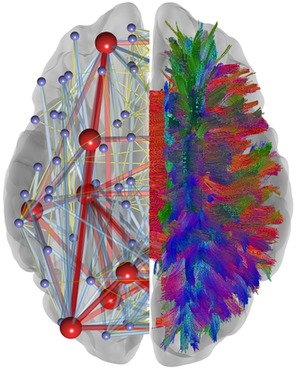
\includegraphics[width=0.5\textwidth]{img/connectome.jpg}
    \caption{Связи между зонами мозга, построенные на основе диффузионно-тензорной МРТ и трактографии нейронных тканей (справа). Коннектом, описывающий связи между зонами мозга. Многие виды нейродегенеративных заболеваний могут быть представлены как особенность подобных графов. \\ Изображение принадлежит Indiana University}
    \label{fig:my_label}
\end{figure}
\newpage\chapter{Обзор литературы}

\indent Многообразие СПО матриц было хорошо изучено в последние десятилетия и нашло широкое применение в задачах анализа медицинских данных, в первую очередь, нейрологических данных \cite{pennec2006riemannian}, \cite{fletcher2007riemannian}, таких как снимки ЭЭГ \cite{barachant2013classification}, функциональной и структурной МРТ. \\

\indent В последнее десятилетие инструменты римановой геометрии использовались в том числе для обработки DTI-изображений (diffusion tensor imaging) \cite{fletcher2007riemannian}, \cite{pennec2006riemannian}. Исследование матрицы ковариации записей ЭЭГ стали классическим подходом в построении интерфейсов «мозг-компьютер»; поскольку матрицы ковариации являются СПО матрицами, к ним возможно применить инструменты римановой геометрии. В задачах классификации ЭЭГ такие методы стали передовыми, показав значительное улучшение результатов по сравнению с существовавшими классическими методами. \cite{barachant2012multiclass}, \cite{barachant2013classification}\\

\indent Матрицы ковариации данных функциональной МРТ также привлекли внимание, учитывая быстрый рост популярности подходов, основанных на построении функциональных графов мозга (функциональных коннектомов) \cite{smith2013functional}. Функциональные коннектомы позволяют представлять функциональные связи мозга на макро-уровне. В последнее время было предложено несколько алгоритмов классификации функциональных коннектомов на основе инструментов римановой геометрии. \\
\indent Slavakis et al.\cite{slavakis2016clustering} представили новаторский подход к отслеживанию шаблонов функциональных связей мозга, варьирующихся во времени. Авторы этой работы использовали геодезические на римановском многообразии и касательные пространства к этому многообразию чтобы сгруппировать свои данных. В этой работе были получены отличные результаты на искусственно сгенерированных коннектомах. Ng et al. \cite{ng2016transport} проецировали матрицы ковариации функциональной МРТ на касательное пространство риманома многообразия с целью снизить взаимное влияние элементов ковариационных матриц; это значительно улучшило точность классификации в задаче с распознаванием четырех активностей на записях функциональной МРТ. \\
\newpage

\indent Сигналы функциональной активации между различными зонами мозга также могут быть представлены как матрицы ковариации, позволяя использовать инструменты римановой геометрии. Однако, этот подход не срабатывает для матриц структурной связности, которые содержат данные об анатомических, а не функциональных связях между регионами мозга. Элементы этих матриц представляют собой число трактов между различными регионами коры головного мозга, обычно построенные на основе диффузионно-взвешенной трактографии. Таким образом, структурные коннектомы являются неориентированными графами, а их матрицы смежности - симметричными матрицами. В противоположность матрицам функциональны связей, матрицы структурных связей не являются определенными. \\

\indent Dodero et al.\cite{dodero2015kernel} предложили метод обхода этого ограничения. Они изучили алгоритмы, основаные на геометрии Римана как для функциональных, так и для структурных коннектомов. Для структурных коннектомов они применили преобразование Лапласа на исходных данных чтобы получить симметричные положительно полуопределенные (СППО) матрицы и регуляризовали полученные матрицы через сложение их с единичной матрицей с маленьким коэффициентом. Их эксперимент на данных из базы данных снимков пациентов с расстройством аутического спектра показал точность классификации 60.76\% и 68\% для функциональных и структурных коннектомов соответственно. % +
% \newpage\chapter{Постановка задачи}

\newpage\chapter{Используемый математический аппарат}

\section{Обозначения}
\begin{itemize}
	\item $M(n)$ – пространство матриц размера $n \times n$ с действительными значениями.
	\item $ Sym(n) = \condset{\bs \in M(n)}{\bs^T \ = \ \bs}$ пространство всех симметричных матриц в $M(n)$.
	\item $ S(n) = \condset{\bs \in Sym(n)}{u^T\bs u > 0, \ \forall u \in \setRn}$ - множество всех симметричных положительно определенных (СПО) матриц размера $n \times n$.
	\item $S^+(n, p) = \condset{\bs \in Sym(n)}{u^T\bs u \geq 0, \ \forall u \in \setRn, \ rk(\bs)=p}$ – множество всех симметричных положительно полуопределенных (СППО) матриц размера $n \times n$ и ранга $p \leq n$. Это обозначение далее будет использоваться только в случае, когда $p<n$.
	\item 
	\item $Gl(n)$ – множество всех обратимых матриц размера $n \times n$ в $M(n)$.
	\item $diag(\lambda_1, \ldots, \lambda_n)$ – матрица размера $n \times n$ со значениями $\lambda_i$ на диагонали.
	\item $Tr(\cdot)$ - оператор следа матрицы
	\item $I = diag(1, \ldots, 1)$ - единичная матрица.
	\item $T_p \manM$ - касательное пространство к многообразию $\manM$ в точке $p$.
\end{itemize}

\section{Общие определения}
\begin{definition}
Норма Фробениуса для матриц: $$\norm{A}{F}^2 = Tr({\bf AA^T}) = \sum{\walls{A_{i,j}}^2}$$. 
\end{definition}
\begin{definition}
Норма $\setL_2$ для вектора ${\bf a}$: $$ \norm{{\bf a}}{2} = \sqrt{\sum_{\substack{i}}|{\bf a_i}|^2}$$
\end{definition}

\begin{definition}
Симметричная матрица $M$ называется положительно полуопределенной, если $\forall x \in \setRn$:
$$ x^T M x \geq 0 $$
$M$ положительно определена, если неравенство строгое $\forall x \neq 0$
\end{definition}

\begin{lemma}
$M$ положительно полуопределенная тогда и только тогда, когда все ее собственные значения $ \forall \lambda_i \geq 0$. Аналогично, $M$ положительно определена, тогда и только тогда, когда $\forall \lambda_i > 0$
\end{lemma}
\begin{proof}
Рассмотрим собственный базис матрицы $M=Q^T \Lambda Q$. Очевидно, что $y^T \Lambda y = \sum_{i} \lambda_i y_i^2 \geq 0 \ \forall y \in \setRn$ тогда и только тогда, когда $\lambda_i \geq 0 \forall i$. Для положительно определенных матриц аналогично.
\end{proof}

\begin{definition}
$n$-мерное топологическое многообразие (без границы) — это Хаусдорфово топологическое пространство, в котором каждая точка имеет открытую окрестность $U$, гомеоморфную открытому подмножеству $n$-мерного Евклидова пространства $\setR^n$.
\end{definition}
Далее будем обозначать $n$-мерное топологическое пространство без границы как «многообразие»
\begin{definition}
Локальная карта многообразия $\manM$ - пара $(U, \phi)$, где $\phi$ - гомеоморфизм из открытого множества $U \subset \manM$ на открытое подмножество $\setR^n$
\end{definition}

\begin{definition}
Множество карт $\set{(U_\alpha \phi_\alpha)}, \alpha \in \Alpha$ ($\Alpha$ - некоторое множество индексов) называется n-мерным $C^k$ атласом, $0 \leq k \leq \infty$ многообразия $\manM$, если:
\begin{itemize}
    \item совокупность всех $U_\alpha$ покрывает $\manM$, т.е. $\manM=\cup _{{\alpha \in A}}U_{\alpha}$.
    \item $ \forall \alpha ,\beta \in A$ таких, что $U_{\alpha }\cap U_{\beta }\neq \varnothing $, отображение:
    $$\phi _{{\alpha }}^{{\beta }}=\phi _{\beta }\circ \phi _{\alpha }^{{-1}}:\phi _{\alpha }(U_{\alpha }\cap U_{\beta })\to \phi _{\beta }(U_{\alpha }\cap U_{\beta })$$
    является гладким отображением класса $C^k$.
\end{itemize}
$ {\displaystyle \phi _{\alpha }^{\beta }}$ называется преобразованием координат точки $m$ с карты  ${\displaystyle (U_{\alpha },\phi _{\alpha })}$ в карту $(U_{\beta },\phi _{\beta })$
\end{definition}

\begin{definition}
Атлас многообразия называется $C^k$-гладким, если ${\displaystyle \phi _{\alpha }^{\beta }}$ является гладким отображением класса гладкости $C^k$
\end{definition}

\begin{definition}
Многообразие называется гладким (или дифференцируемым), если оно наделено $C^k$-гладкой структурой, задаваемой $C^k$-гладким атласом
\end{definition}

Для гладких многообразий можно ввести понятия касательного вектора, касательного пространства, длины кривой.
\section{Геометрия Риманова многообразия}

В этом разделе описаны принципы и инструменты геометрии многообразия симметричных положительно определенных матриц (Риманова многообразия.)

\subsection{Риманово многообразие}

\begin{definition}
Римановым называется многообразие $\manM$ с заданным на нем  $m \in \manM$ скалярным произведением $\left< \cdot \right>_\bc$ касательных векторов в касательном пространстве $T_p \manM$, таким, что оно гладко зависит от $p$.
\end{definition}

\begin{definition}
Риманова метрика $g$ на многообразии $\manM$ – семейство всех скалярных произведений на всех касательных пространствах
\end{definition}

\indent Далее будем рассматривать многообразие симметричных положительно определенных (СПО) матриц как пример риманова многообразия. Имеем следующие свойства: 
\begin{lemma}
Свойства пространства $S(n)$:
\begin{itemize}
	\item $\forall \ \bs \in S(n),\ det(\bs) > 0$
	\item $\forall \ \bs \in S(n),\ \bs^{-1} \in S(n)$
	\item $\forall \ (\bs_1, \bs_2) \in S(n)^2,\ \bs_1 \bs_2 \in C(n)$
\end{itemize}
\end{lemma}

\indent СПО матрицы из семейства $S(n)$ всегда диагонализуемы и имеют строго положительные действительные собственные значения. Для СПО матриц в $S(n)$ матричная экспонента $\bs$ задается через собственные значения сингулярно-векторного разложения матрицы $\bs$:
$$ \bs = {\bf U} \ diag(\sigma_1, \ldots, \sigma_n) \ {\bf U}^T, $$
где $\sigma_1 > \sigma_2 > \ldots > \sigma_n$ - собственные значения и ${\bf U}$ - матрица собственных векторов $\bs$. 
\begin{definition}
Матричная экспонента $\bs \in S(n)$: 
 $$ exp(\bs) = {\bf U} \ diag(exp(\sigma_1), \ldots, exp(\sigma_n)) \ {\bf U}^T $$
\end{definition}

\begin{definition}
Логарифм матрицы $\bs \in S(n)$:
$$ log(\bs) = {\bf U} \ diag(log(\sigma_1), \ldots, log(\sigma_n)) \ {\bf U}^T  $$ \\
\end{definition}
\indent Взятие логарифма матрицы $\bs \in S(n)$ является обратной операцией к взятию матричной экспоненты.

\begin{lemma}
Свойства пространства $S(n)$, связанные с матричными экспонентой и логарифмом:
\begin{itemize}
	\item $\forall \ \bs \in S(n),\ log(\bs) \in Sym(n)$
	\item $\forall \ \bc \in Sym(n),\ exp(\bc) \in S(n)$
	    
\end{itemize}
\end{lemma}

\subsection{Риманова метрика}
Пространство СПО матриц $S(n)$ – это риманово многообразие $\setM$, следовательно, оно дифференцируемо. Производная матрицы $\bs$ на многообразии лежит в векторном пространстве $T_{\bs}$, являющимся касательным пространством к этой точке. Касательное пространство лежит в пространстве $Sym(n)$. Многообразие и касательное пространство имеют размерность $m = n(n+1)/2$ \cite{faraut1994analysis} \\
\indent Для каждого касательного пространства определено скалярное произведение $\left< \cdot \right>_\bc$, гладко меняющееся от точки к точке. Натуральная метрика на многообразии СПО матриц определена локальным скалярным произведением: 
\begin{equation} \label{nmetr}
	 \inprod{C_1}{C_2}{\bs} = Tr(C_1\bs^{-1}C_2\bs^{-1})
\end{equation}

\indent Через скалярное произведение можем задать норму касательных векторов: \begin{equation} \label{nnorm}
	 \norm{\bc}{\bs}^2 = \inprod{\bc}{\bc}{\bs} = Tr(\bc\bs^{-1}\bc\bs^{-1})
\end{equation}

\subsection{Геодезические в римановом пространстве}
Обозначим $ \Gamma(t): \ [a,b] \rightarrow S(n) : \bs^i=\bs^i(t), i=\set{1, \ldots, n}, a \leq t \leq b$ - произвольная кривая риманова многообразия $(\manM, g)$. В любой точке этого пути касательный вектор определяется как: 
$$ v(t) =(\dot{\bs}^1(t), \ldots, \dot{\bs}^n(t) )$$
$$ |v(t)|_\bs = \sqrt{\left< v,v \right>_g\rvert_\bc} $$
Длина этой кривой определяется как: 
\begin{equation}
	L(\Gamma(t)) = \int_{a}^{b} \norm{\dot{\Gamma}(t)}{\Gamma(t)} dt = \int_{a}^{b} \sqrt{g_{ik}(\bs)\dot{\bs}^i\dot{\bs}^k} dt, \\
	g_{ik} = \left< \frac{\partial}{\partial \bs^i}, \frac{\partial}{\partial \bs^k} \right >
\end{equation}
где используется норма, определенная в предыдущем разделе формулой \eqref{nnorm}. Путь минимальной длины, соединяющий две точки многообразия, называется геодезической, и риманово расстояние между двумя точками определяется как длина этого пути. Натуральная метрика \eqref{nmetr} задает геодезическое расстояние.

\begin{equation} \label{geodd}
	\delta_{spd}(\bs_1,\bs_2) = \norm{log(\bs_1^{-1}\bs_2)}{F} = \Big{[} \sum_{i=1}^{n} log^2 \lambda_i \Big{]}^{1/2},
\end{equation} 

где $\lambda_1, \ldots, \lambda_n$ - действительные собственные значения $\bs_1^{-1}\bs_2$. Главные свойства риманова геодезического расстояния:
\begin{itemize}
	\item $\delta_{spd}(\bs_1,\bs_2) = \delta_{spd}(\bs_2, \bs_1)$
	\item $\delta_{spd}(\bs_1^{-1},\bs_2^{-1}) = \delta_{spd}(\bs_1,\bs_2)$
	\item $\delta_{spd}(\bw^T\bs_1\bw,\bw^T\bs_2\bw) = \delta_{spd}(\bs_1,\bs_2) \ \forall \ \bw \in Gl(n)$
\end{itemize}


\subsection{Экспоненциальная проекция}
Для каждой точки $\bs \in S(n)$ можно задать касательное пространство $\tau_C\mathcal{M}$, образованное множеством векторов, касательных к $\bs$. Каждый касательный вектор $\bc_i$ может рассматриваться как производная в точке $t=0$ от геодезической $\Gamma_i(t)$ между $\bs$ и экспоненциальной проекцией $\bs_i=Exp_\bs(\bc_i)$ \\
% \begin{figure}[h]
% 	\centering
% 	\includegraphics[width=0.7\textwidth]{./img/projection}
% 	\caption{Многообразие $\mathcal{M}$ и соответствующее касательное пространство $\tau_C\mathcal{M}$ в точке $\bc$}
% \end{figure} \\
\indent Экспоненциальная проекция определяется как:
\begin{equation}
	Exp_\bs(\bc_i) = \bs_i = \bs^{1/2}exp(\bs^{-1/2}\bc_i\bs^{-1/2})\bs^{1/2}
\end{equation}
\indent Обратная проекция определяется как логарифмическая проекция вида:
\begin{equation} \label{logpr}
	Log_\bs(\bs_i) = \bc_i = \bs^{1/2}log(\bs^{-1/2}\bs_i\bs^{-1/2})\bs^{1/2}
\end{equation}
\indent В терминах проекции можно ввести эквивалетное определение риманового расстояния:
$$ \delta_R(\bs_1,\bs_2) = \norm{Log_\bs(\bs_i)}{\bs} = \norm{\bc_i}{\bs} = \\ $$
$$	= \norm{upper(\bs^{-1/2}Log_\bs(\bs_i)\bs^{-1/2}}{2} = \norm{c_i}{2}, $$
где $upper(\cdot)$ - оператор, оставляющий верхнетреугольную часть симметричной матрицы и векторизующий ее, добавляя единичный вес диагональным элементам и $\sqrt{2}$ вес не-диагональным. $c_i$ здесь - $m$-мерный вектор $upper(\bs^{-1/2}Log_\bs(\bs_i)\bs^{-1/2}$ нормализованного касательного пространства.
\section{Геометрия пространства СППО матриц}
\subsection{Метрика на многообразии СППО матриц}
Можем выразить $\spn$: 
$$ \spn \cong (V_{n,p} \times S(p))/O(p) $$

Размерность $\spn$ есть $dim(V_{n,p} \times S(p)) - dim(O(p))=pn-p(p-1)/2$. \\
Если $(U, R^2) \in V_{n,p} \times S(p)$ представляет $A \in \spn$, то можно выразить касательные вектора $T_A\spn$ бесконечно малыми изменениями $(\Delta, D)$, где 
$$ \Delta = U\botB, \ B \in \setR^{(n-p) \times p} $$
$$ D = RD_0R $$
такие, что $U \bot \in V_{n, n-p}, \ U^TU\bot = 0$ и $D_0 \in Sym(p) = T_IS(p)$. Тогда метрика $\spn$ может быть задана как сумма бесконечно малых расстояний в $Gr(p,n)$ и $S(p)$:
\begin{equation}\label{spsd_metric}
     g_{(U, R^2)}((\Delta_1, D_1), (\Delta_2, D_2)) = Tr(\Delta_1^T \Delta_2) + k \ Tr(R^{-1}D_1R^{-2}D_2R^{-1}), \ k>0
\end{equation}
Следующая теорема доказывает, что введение этой метрики наделяет $\spn$ римановой структурой
\begin{theorem}
Пространство $ $\spn$ \cong (V_{n,p} \times S(p))/O(p) $, наделенное метрикой \eqref{spsd_metric} является римановым многообразием с горизонтальным пространством 
$$ \manH_{(U, R^2)} = \set{(\Delta, D):\ \Delta=U\bot B, \ B \in \setR^{(n-p) \times p},\ D=RD_0R, \ D_0 \in Sym(p)} $$
Более того, эта метрика инвариантна относительно ортогональных преобразований, масштабирования и псевдоинверсии.
\end{theorem}
Доказательство этой теоремы может быть найдено в \cite{bonnabel2009riemannian}
\newpage
\subsection{Геодезические на многообразии СППО матриц}
В этой секции рассматривается построение геодезических, соединяющих матрицы $A,B \in \spn$. \\
Пусть $V_A, V_B \in V_{n,p}$ – две матрицы, являющиеся линейными оболочками, порожденными $A, B$. Сингулярное разложение $V_B^TV_A$ порождает $O_A, O_B \in \setR^{p \times p}$ такие, что
\begin{equation} \label{OVVO}
      O_A^TV_A^TV_BO_B = diag(\sigma_1, \ldots, \sigma_p), 1 \geq \sigma_1 \geq \ldots \geq \sigma_p \geq 0
\end{equation}
$\sigma_i =  \cos \theta_i$ - косинусы углов $0 \leq \theta_1 \leq \ldots \leq \theta_p \leq \pi/2$ между двумя подпространствами.\\
Корневые вектора $ U_A=(u_1^A, \ldots, u_p^A) = V_AO_A $ и $U_B=(u_1^B, \ldots, u_p^B) = V_BO_B$ дают формулу грассмановской геодезической, соединяющей $range(A)$ и $range(B)$
\begin{equation}
     \label{grassman_geodesics}
     U(t) = U_A \cos(\Theta t)V + X \sin(\Theta t)
\end{equation}
где $\Theta = diag(\theta_1, \ldots, \Theta_p)$, а $X$ - нормализованная проекция $V$ на пространство столбцов $U\bot$, т.е. 
$X=(I-U_AU_A^T)U_BF$, где $F$ - псевдоинверсия матрицы $diag(\sin(\theta_1), \ldots, \sin(\theta_p))$. \\
Соответствующая геодезическая $R^2(t)$ в $S(p)$ должна соединять $R_A^2=U_A^TAU_A$ и $R_B^2=U_B^TBU_B$ :

\begin{equation}
     \label{p-geodesics}
     R^2(t) = R_A \exp(t\log R^{-1}_AR^2_BR^{-1}_A)R_A
\end{equation}

Таким образом геодезическая задается следующим выражением:
\begin{equation}
     \label{spsd_geodesics}
     \gamma_{A \rightarrow B}(t) = U(t)R^2(t)U^T(t)
\end{equation}
Геодезические, исходящая из любой точки, сохраняет ранг, симметричность и положительную определенность матрицы $UR^2U^T$, формируют покрытие $S^+(n,p)$, определены на $\spn$ $\forall t \in \setR$ для любого касательного вектора. \\

\subsection{Расстояние между СППО матрицами}
\begin{theorem}
Сингулярное разложение \eqref{OVVO} и геодезические кривые \eqref{grassman_geodesics} и \eqref{p-geodesics} задают кривую в $\spn$:
$$ \gamma_{A \rightarrow B}(t) = U(t)R^2(t)U^T(t) $$
со следующими свойствами:
\begin{itemize}
    \item $\gamma_{A \to B}(\cdot)$ соединяет $A$ и $B$ в $\spn$ так, что $\gamma_{A \to B}(0) = A, \ \gamma_{A \to B}(1)=B$ и $\gamma_{A \to B}(t) \in \spn \forall t \in [0, 1]$
    \item Кривая $(U(t), R^2(t))$ является горизонтальным сдвигом $\gamma_{A \to B}(t)$ и является геодезической в структурном пространстве $V_{n,p} \times S(p)$
    \item Квадратичная длина $\gamma_{A \to B}$ на римановом многообразии $(\spn, g)$ задается следующим выражением:
    \begin{equation}
        \label{spsd-distance}
         l^2(\gamma_{A \to B}) = ||\Theta||_F^2 + k ||\log R_A^{-1} R_B^2 R_A^{-1}||_F^2
    \end{equation}
    Она инвариантна относительно псевдоинверсии, ортогональных преобразований и масштабирования.
\end{itemize}
Более того, кривая $\gamma_{A \to B}$ уникальна, если $(p-1)$ угол между пространствами удовлетворяет $\theta_{p-1} \neq \pi/2$
\end{theorem}
Доказательство этой теоремы подробно рассмотрено в \cite{bonnabel2009riemannian} % +
\newpage\chapter{Существующий подход}
\indent Большинство методик классификации СПО матриц можно разделить на две группы:
\begin{enumerate}
    \item Ядерные методы, основанные на высчитаной заранее матрице расстояний между СПО матрицами
    \item Двухшаговые алгоритмы, состоящие из (1) проекции всех СПО матриц на подходящее касательное пространство и (2) классификации получившихся векторов линейными алгоритмами классификации (такими как логистическая регрессия или линейный диксриминантный анализ)
\end{enumerate}

\section{Ядерные методы}
\indent Ядерные методы в $\setR^n$ крайне эффективны в задачах машинного обучения и компьютерного зрения, требующих распознавания нелинейных структур в данных. Поэтому ядерные методы являются достаточно распространенным подходом к классификации коннектомов, так как они могут обрабатывать коннектомы как графы, тогда как другие методы обычно требуют конвертации коннектомов в векторы (например, векторы глобальной метрики на графах). Основная идея ядерных методов состоит в том, чтобы отразить данные в пространство большей размерности. В случае данной работы это отображение является построением матрицы расстояний между коннектомами, на основе введенного расстояния или подобного расстоянию измерения между коннектомами. Например, расстояние, основанное на сходстве разбиения структурных коннектомов на группы было представлено в \cite{kurmukov2016classification}.\\
\indent Методы, работающие с римановым многообразием, используют метрику на $\manM$. Когда выбрано расстояние $\delta_{spd}(\bs_i, \bs_j)$, алгоритм классификации не вызывает затруднений. 
\subsection{Положительно определенные ядра на многообразиях}
\indent В $\setR^n$ гауссовское ядро может быть выражено следующим образом с использованием евклидова расстояние между точками $x_i, x_j$:
$$ K(x_i, x_j) = exp\Big(\frac{||x_i - x_j||^2}{2\sigma^2}\Big) $$
Чтобы определить ядро на римановом многообразии, нужно заменить евклидово расстояние на более точное геодезическое расстояние на многообразии. Однако не все геодезические позволяют построить положительно определенное ядро. \\
\indent Начнем с определения положительно и отрицательно определенных ядер \cite{berg1984harmonic}
\begin{definition}
Пусть ${\mathcal X}$ – непустое множество. Функция $f: ({\mathcal X} \times {\mathcal X}) \Rightarrow \setR$ называется положительно (отрицательно) определенным ядром тогда и только тогда, когда $f$ симметрична и $$ \sum_{\substack{i,j}}^m c_ic_jf(x_i, x_j) \geq 0 (\leq 0) $$
для любого $m \in \setN, \set{x_1, \ldots, x_m} \subset \manX, \set{c_1, \ldots, c_m} \subset \setR$, причем для отрицательно определенного ядра $\sum_{i=1}^m c_i=0$
\end{definition}
\begin{theorem}
Пусть $(\manM, g)$ - метрическое пространство и определим отображение $K:(\manM \times \manM) \Rightarrow \setR$ следующим образом:
$$ K(x_i, x_j) = exp\Big(\frac{-d^2(x_i, x_j)}{2\sigma^2}\Big) $$
В таком случае $K$ является положительно определенным ядром для любых $\sigma>0$ тогда и только тогда, когда существует линейное пространство $\Nu$ с заданным на нем скалярным произведением и функция $\psi: \manM \Rightarrow \Nu$ такая, что $d(x_i, x_j)=\norm{\psi(x_i) - \psi(x_j)}_{\Nu}$
\end{theorem}
Доказательство этой теоремы рассмотрено в \cite{jayasumana2013kernel}
Следующая теорема была введена в \cite{schoenberg1938metric}
\begin{theorem}\label{schoenberg}
Пусть $\manX$ - непустое множество и $f: (\manX \times \manX) \Rightarrow \setR$ - функция. Ядро $exp(-\gamma f(x_i,x_j))$ положительно определено для любых $t>0$ тогда и только тогда, когда $f$ отрицательно определена.
\end{theorem}
Детальное доказательство теоремы \eqref{schoenberg} можно найти в главе 3, теорема 2.2 в работе \cite{berg1984harmonic}.

\indent Мы можем построить ядро следующим образом:
\begin{equation}\label{kernel}
    K_{spd} = exp(-\gamma \delta_{spd}(\bs_i, \bs_j),
\end{equation}

где $\gamma>0$ - параметр. Поскольку $\delta_{spd}$ является метрикой, ядро $K_P$ положительно определено. Таким образом, можем использовать алгоритм машины опорных векторов \cite{scholkopf2001learning} для классификации на основе $K_{spd}$ 

\section{Классификация в касательном пространстве}
 \indent Многие эффективные алгоритмы (например, LDA, SVM) основаны на основаны на проекции данных на гиперплоскости. Соответственно, они не могут быть реализованы напрямую на римановом многообразии. Реализация более простых алгоритмов может осуществляться с использованием пространства $T_\bc \manM$, касательного к рассматриваемому многообразию.  \\
\indent Принципиальный вопрос в этом подходе заключается в выборе опорной точки $\bs$, которая должна находиться достаточно близко к точкам обучающего множества $\set{\bs_i, y_i}_{i=1}^n$. Стандартным вариантом опорной точки является геометрическое среднее всех матриц, которое задается следующим образом:
 $$ \bs_m = Mean(\bs_1, \ldots, \bs_n) = arg \min_{\substack{\bs \in S(n)}}\sum_{\substack{i=1}}^n \delta_{spd}^2(\bs, \bs_i) $$
 \indent Это среднее также называется геодезическим средним. Каждая ковариационная матрица затем проецируется на касательное пространство, формируя $m$-мерные векторы, где $m=\frac{n(n+1)}{2}$:
 $$ \bc_i = upper(\bs_m^{-\frac{1}{2}}Log_{\bs_m}(\bs_i)\bs_m^{-\frac{1}{2}}) $$
 \indent Эффективный алгоритм вычисления среднего для множества СПО матриц был представлен в \cite{barachant2013classification} \\
 \indent Таким образом мы переходим из нелинейного пространства, в котором невозможно использовать евклидово расстояние, в линейное с помощью заведомо линейного преобразования - проекции.
 % +
\newpage\chapter{Предложенный подход}

В этой главе рассмотрим бинарную классификацию матриц структурных коннектомов. В качестве входных данных имеем множество пар данных (матриц смежности) и ответов (меток классов): $ \set{\ba_i, y_i}_{i=1}^N, \ \ba_i \in Sym(n), y_i \in \set{0,1}$, где $n$ – число вершин в каждом графе коннектома.

\section{Конвертация структурных коннектомов в СППО матрицы}
Первый шаг алгоритма состоит в конвертации структурных коннектомов в симметричные положительно полуопределенные матрицы. В работе \cite{dodero2015kernel} было предложено использовать для этого лапласианы матриц данных.

\begin{definition}
Пусть $m$ - число ребер, $n$ - чисто вершин графа. Тогда матрица смежности $\nabla = \nabla_G$ - матрица размера $m \times n$ следующего вида:
\begin{equation*} 
\nabla_{e,v} = 
\begin{cases}
1 & \quad \text{если } e=(v,w) \text{ и } v<w \\
-1 & \quad \text{если } e=(v,w) \text{ и } v>w \\
0 & \quad \text{иначе}\\
\end{cases}
\end{equation*} 
\end{definition}

\begin{lemma}
$L_G = \nabla^T \nabla$
\end{lemma}
\begin{proof}
$[\nabla^T\nabla]_{ij}=$(i-й столбец $\nabla$) $\cdot$ (j-й столбец $\nabla$)=$\sum_e\big( [\nabla]_{e,v_i} \big)\big( [\nabla]_{e,v_j} \big)$, что дает три возможных случая:
\begin{itemize}
    \item $i=j$
    $$ [\nabla^T\nabla]_{ij} = \sum_{\substack{e}}\Big( [\nabla]_{e,v_i} \Big)^2 = \sum_{\substack{e смежные с v_i}}1 = deg(i) $$
    \item $i \neq j$ и между вершинами $v_i, v_j$ нет ребра
    $$ [\nabla^T\nabla]_{ij} = \sum_{\substack{e}}\Big( [\nabla]_{e,v_i} \Big)\Big( [\nabla]_{e,v_j} \Big) = 0,$$
    поскольку ни одно ребро не смежно как минимум с одной из вершин $v_i, v_j$
    \item  $i \neq j$ и между вершинами $v_i, v_j$ есть ребро
    $$ [\nabla^T\nabla]_{ij} = \sum_{\substack{e}}\Big( [\nabla]_{e,v_i} \Big)\Big( [\nabla]_{e,v_j} \Big) = \Big( [\nabla]_{e',v_i} \Big)\Big( [\nabla]_{e',v_j} \Big)$$
\end{itemize}
\end{proof}

\begin{corollary*}
$$ x^T L_G x = ||\nabla x||^2  = \sum_{\substack{(i,j) \in E}} (x_i-x_j)^2,$$
где $E$ - множество ребер графа
\end{corollary*}

Таким образом, лапласиан является симметричной положительно полуопределенной матрицей. В предложенном подходе будем использовать нормализованные лапласианы.
Преобразование данных задается следующим образом:
$$ \bx_i = \bd_i^{-\frac{1}{2}} (\bd_i - \ba_i) \bd_i^{-\frac{1}{2}}, $$
где $\bd_i$ – диагональная матрица степеней взвешенных вершин: $ \bd_i \rvert_{k,k} = \sum_{\substack{l}} \ba_i\rvert_{k,l}$.

\section{Классификация на основе $\delta_{spsd}$}

Обобщение подхода, основанного на использовании ядерных функций, не вызывает затруднений - мы можем использовать $\delta_{spsd}$, заданное формулой \eqref{spsd-distance}, чтобы построить ядро (матрицу расстояний между полученными лапласианами). \\
Адаптация методов, основанных на проекции на касательное пространство, в случае многообразия СППО матриц, однако, гораздо сложнее, поскольку мы не можем построить касательное пространство к среднему всех СППО матриц. Чтобы обойти это ограничение, в этой работе использован алгоритм снижения размерности Isomap \cite{tenenbaum2000global} на матрицах данных  $\bx_i, i \in \set{1, \ldots, n}$, как было предложено в \cite{krivov2016dimensionality}.
Таким образом, в предложенном подходе основной упор делается на алгоритмы, основанные на ядерных функциях. % +
\newpage\chapter{Эксперименты}

\section{Данные}
\indent В качестве экспериментальных данных использовалась база МРТ-снимков Alzheimer's Disease Neuroimaging Initiative. Данные содержат снимки пациентов в различными стадиями развития болезни Альцгеймера: 
\begin{enumerate}
    \item здоровые пациенты: NC (normal cohort)
    \item пациенты с умеренными когнитивными нарушениями: EMCI (early mild cognitive impairment)
    \item пациенты с выраженными когнитивными нарушениями: LMCI (late mild cognitive impairment)
    \item пациенты с болезнью Альцгеймера: AD (Alzheimer's disease)
\end{enumerate}

\indent Таким образом, решается задача классификации для четырех классов. \\
База данных состоит из снимков 228 пациентов, всего 748 снимков. Средний возраст испытуемых на момент начала эксперимента: $72.9 \pm 7.4$ лет. Среди пациентов 96 женщин и 132 мужчины. Распределение по классам следующее: 50 пациентов AD, 43 LMCI, 77 EMCI, 61 NC. \\
\indent T1-взвешенные снимки были обработаны с помощью FreeSurfer \cite{fischl2012freesurfer}. В обработке использовался атлас Desikan-Killiany \cite{desikan2006automated}, содержащий 68 регионов коры головного мозга. DWI (diffusion weighted imaging) снимки были скорректированы с учетом искажений, вызванных движением. Вероятностная трактография была выполнена с использованием модуля локального трекинга (LocalTrecking) фреймворка Dipy \cite{garyfallidis2014dipy} с ограничением на обратную сферическую свертку (constrained spherical deconvolution, CSD \cite{tax2014recursive}). Нервные связи длинее 5 мм, с обоих концов пересекающие поверхность коры, были удалены. Веса ребер графа, представляющего связность регионов, были высчитаны в соответствии с числом детектированых нервных связей.

\section{Влияние ранга матриц данных на результат классификации}
\indent В этом разделе рассматривается влияние ранга матриц данных на расстояния между ними и точность классификации. В частности, проверяется гипотеза о том, может ли искусственное снижение ранга повлиять на погрешность трактографии, допускаемую при исходной обработке МРТ-снимков.\\
\indent Для искусственного снижения ранга использовалось сингулярное разложение матриц $$\bx_i = U*S*V, \bx_i \in S^+(n,p),$$ где $S$ - диагональная матрица собственных значений $\bx_i$. Пусть $k \in \setN$ - ранг матрицы, который мы хотим получить после преобразования. Для снижения ранга заменяем $p-k$ минимальных собственных значений нулями: $$ S_{j,j} = 0, j \in \set{1, \ldots, p-k} $$
Можем видеть, что матрица расстояний меняется практически линейно в зависимости от ранга:
\begin{figure}[!h]
\minipage{0.32\textwidth}
  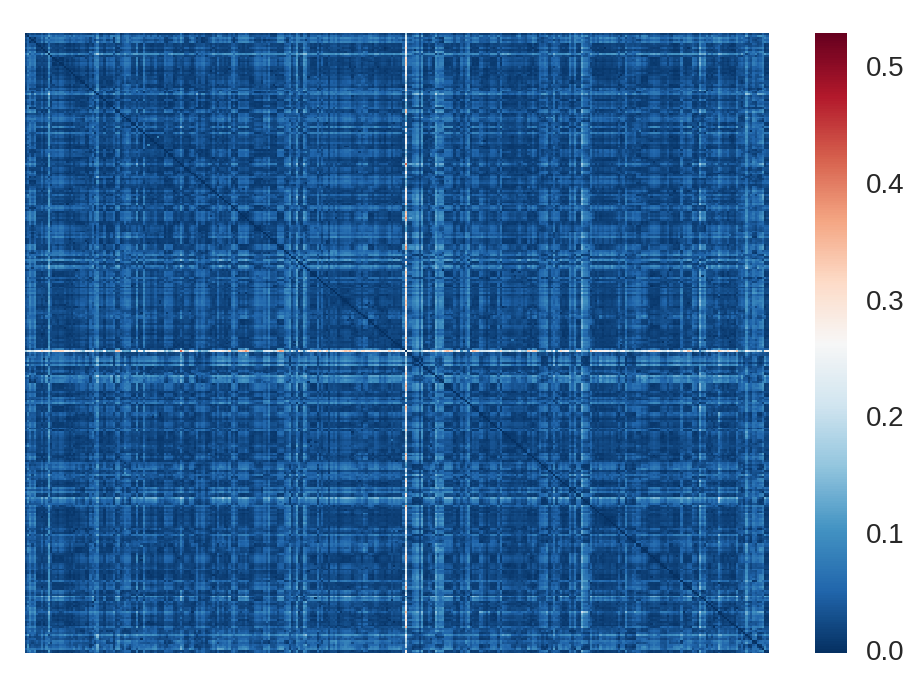
\includegraphics[width=\linewidth]{img/diff_drop_4.png}
  \caption{}
\endminipage\hfill
\minipage{0.32\textwidth}
  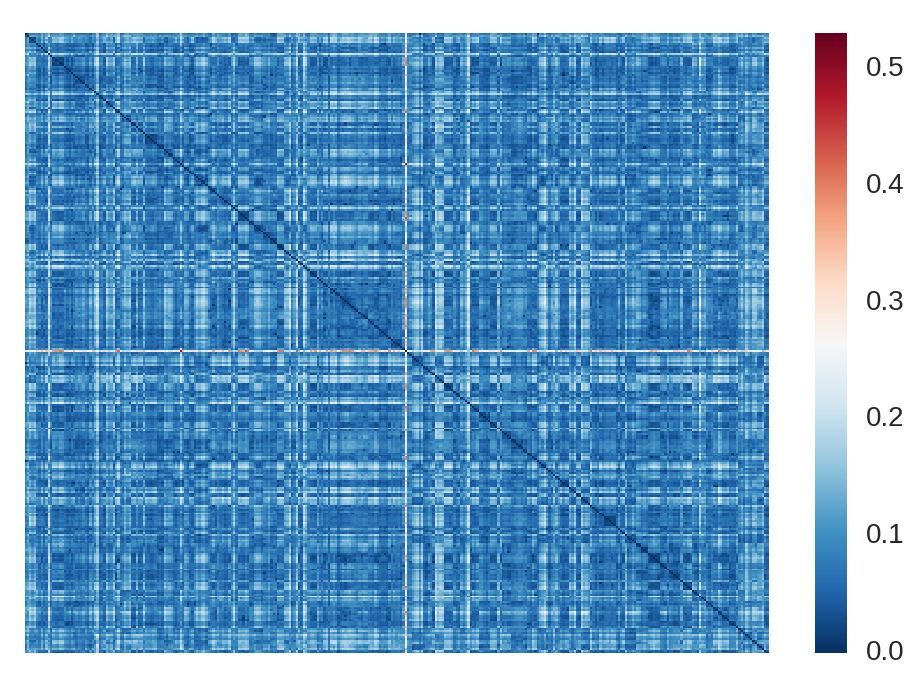
\includegraphics[width=\linewidth]{img/diff_drop_8.png}
  \caption{}
\endminipage\hfill
\minipage{0.32\textwidth}
  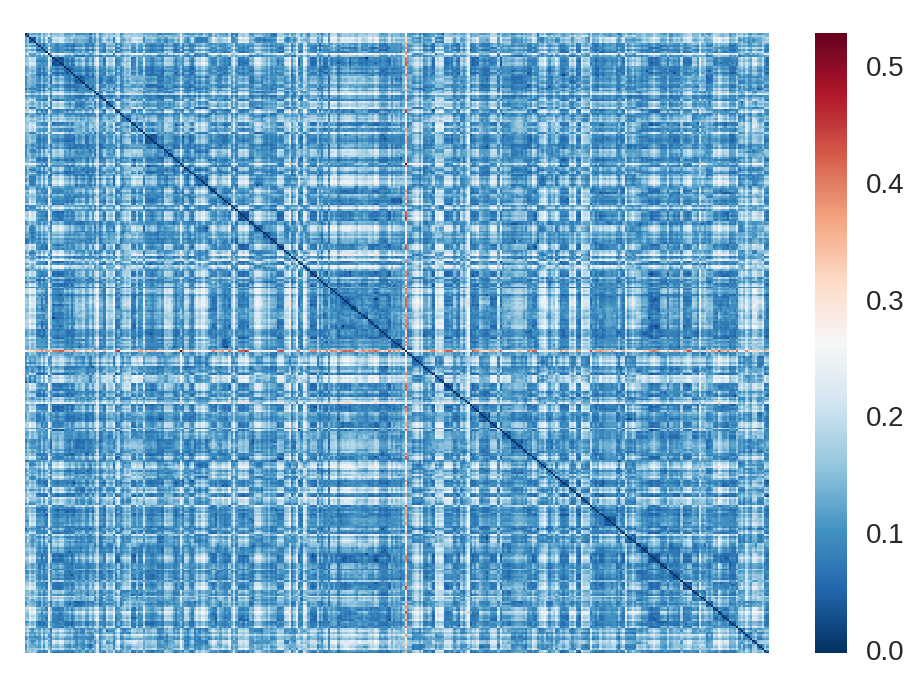
\includegraphics[width=\linewidth]{img/diff_drop_12.png}
  \caption{}
\endminipage
\caption{Изменение матрицы расстояний между матрицами данных при снижении ранга матриц данных на 4 (7.1), 8 (7.2) и 12(7.3)}
\end{figure}

\section{Базовые результаты}
\indent В качестве ориентировочных результатов использовались результаты двух методов:
\begin{enumerate}
    \item Как простейший метод, использовался алгоритм ядерной опорной машины векторов с ядром на основе $L2$ расстояний между матрицами данных
    \item Ядерный подход, предложенный в \cite{dodero2015kernel}. После высчитывания лапласианов матриц данных, к ним были добавлены единичные матрицы с коэффициентом $1e-3$ (алгоритм устойчив к выбору этого коэффициента, как предположено в \cite{dodero2015kernel}). Далее было высчитано логаримфированное евклидово расстояние между матрицами и классифицировано ядерным SVM с гауссовским ядром. Подробно алгоритм описан в \cite{dodero2015kernel}
\end{enumerate}

\section{Постановка эксперимента}
\indent В эксперименте проверялись результаты двух методов, предложенных прошлой главе:
\begin{enumerate}
    \item Ядерный SVM на основе «метрики» $\delta^k_{spsd}$
    \item Снижение размерности СППО матриц с помощью Isomap с последующей классификацией в пространстве меньшей размерности с помощью логистической регрессии с $l2$ регуляризацией.
\end{enumerate}

\begin{itemize}
    \item Для ядерных методов использовался поиск по множеству значений параметра $\gamma$ формулы \eqref{kernel} и параметру регуляризации $C$ машины опорных векторов.
    \item Для алгоритма Isomap использовался поиск по множеству значений итоговой размерности и числа соседей.
    \item Для логистической регрессии использовался поиск по параметру регуляризации.
    \item Для всех алгоритмов использовался поиск по значению коэффициента $k$ формулы \eqref{spsd-distance}
\end{itemize}
Поскольку в теоретических исследованиях не дается рекомендаций по выбору $k$ в \eqref{spsd-distance} \cite{bonnabel2009riemannian}, то выбор $k$ был произведен с помощью вычислительного эксперимента.
 
\indent Используемые множества значений параметров представлены в таблице ниже.\\
 
\begin{table}[!h]
\centering
\begin{tabular}{lll}
\hline
\rowcolor[HTML]{EFEFEF} 
Алгоритм                & Параметр                            & Множество значений                                                                                                                                                                                                        \\ \hline
Ядерные методы          & Коэффициент $\gamma$                & $\set{10^{0.25i}}_{i=-12}^4, \ i\in \setN$
     \\ 
Ядерные методы          & Параметр регуляризации SVM          & 0.1, 1, 5, 10, 50                                                                                                                                                                                                         \\
Isomap                  & Размерность итогового пространства  & 2, 4, 6, 8, 10                                                                                                                                                                                                            \\
Isomap                  & Число соседей                       & 60, 100, 150, 200, 250                                                                                                                                                                                                    \\
Логистическая регрессия & Параметр регуляризации              & $\set{10^{i}}_{i=-5}^3, \ i \in \setN $                                                                                                                                                                      \\
Все алгоритмы           & Коэффициент $k$ в $\delta_{spsd}^k$ & $\set{10^i}_{i=-4}^2, \ i \in \setN$ 
\end{tabular}
\caption{Множества значений параметров, использовавшиеся в переборе}
\end{table}

\indent Параметры были подобраны с использованием 10-фолдной кросс-валидации. В качестве алгоритма кросс-валидации использовался KFold, позволяющий гарантированно определять снимки одного пациента в один и тот же фолд. \\
Для лучших параметров кросс-валидация была повторена 10 раз на разных разбиениях данных, чтобы оценить эффективность алгоритмов.

\indent В качестве метрики качества во всех экспериментах использовалась площадь под ROC-кривой (ROC AUC)
\begin{definition}
\indent ROC-кривая – кривая, отображающая соотношение True positive rate и False positive rate при варьировании решающего правила классификатора
\end{definition}
\indent В интегральном выражении площадь под ROC-кривой задается следующим выражением:
\begin{equation}
\label{roc-auc}
    AUC =\int _{\infty }^{-\infty }{TPR}(T)\left(-FPR'(T)\right)\,dT=\int _{-\infty }^{\infty }\int _{-\infty }^{\infty }I(T'>T)f_{1}(T')f_{0}(T)\, \ dT'\,dT=P(X_{1}>X_{0})
\end{equation}

\indent Алгоритм построения ROC-кривой и явного вычисления ROC AUC представлен ниже\\
\begin{algorithm}[H]
    $m^- = \sum_{i=1}^n [y_i=-1]\;
    m^+ = \sum_{i=1}^n [y_i = +1]$\;
    $(FPR_0, \ TPR_0) = (0,0)$\;
    $AUC = 0$\;
    \For{$i=1, \ldots, N$}{
        \If{$y_i=-1$}{
            $FPR_i = FPR_{i-1}+\frac{1}{m^-}$\;
            $TPR_i = TPR_{i-1}$\;
            $AUC = AUC + \frac{1}{m^-}TPR_i$\;
        }
        \else{
            $FPR_i = FPR_{i-1}$\;
            $TPR_i = TPR_{i-1} + \frac{1}{m^+}$
        }
    }
\end{algorithm}
 % +
\newpage\chapter{Результаты}
Результаты попарной классификации для пар классов (AD, NC), (AD, LMCI), (LMCI, EMCI), (EMCI, NC), полученные на базовых алгоритмах, представлены в таблице ниже:
\begin{table}[h]
\centering
\begin{tabular}{lll}
\rowcolor[HTML]{EFEFEF} 
\hline
Пара классов & SVM + L2 расстояние & SVM + SPD регуляризация \\
\hline
(AD, NC)     & 77.2 $\pm$ 0.99     & 80 $\pm$ 0.54       \\
(AD, LMCI)   & 65.5 $\pm$ 1.6      & 68.8 $\pm$ 0.81     \\
(LMCI, EMCI) & 44.7 $\pm$ 2.9      & 47.8 $\pm$ 2.4      \\
(EMCI, NC)   & 50.4 $\pm$ 1.8      & 53.9 $\pm$ 1.6     
\end{tabular}
\caption{Результаты классификации базовых алгоритмов, метрика качества – ROC AUC \eqref{roc-auc}}
\end{table}

На рисунке ниже представлена зависимость качества классификации предложенных в работе методов в зависимости от параметра $k$ в формуле расстояния на СППО многообразии \eqref{spsd-distance}
\begin{figure}[h!]
\centering
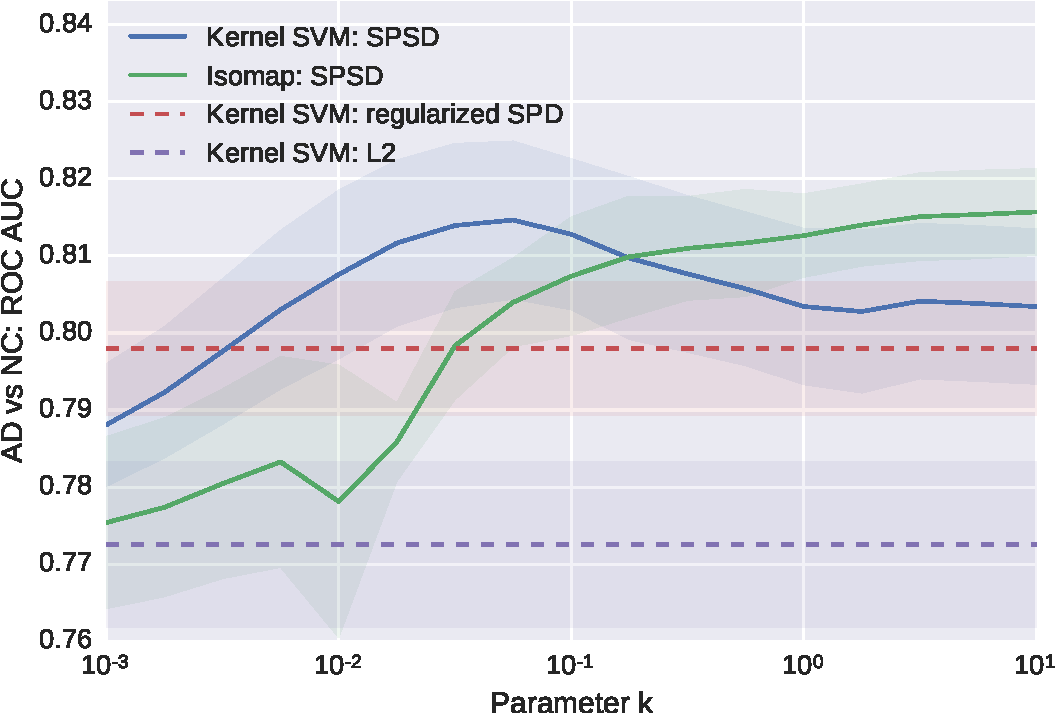
\includegraphics[width=0.8\textwidth]{img/k_dep.pdf}\label{fig:clf_quality}
\caption{Качество классификации как функция от параметра $k$ в \eqref{spsd-distance}. Четыре линиис соответствуют средним значениям площади под ROC-кривой, оцененной с помощью 10-фолдной групповой кросс-валидации. Прозрачные области соответствуют среднеквадратичному отклонению}
\end{figure}

\newpage Подход с использованием снижения размерности СППО матриц изначально был применен для проекции данных на двумерное пространство, чтобы получить возможность визуально оценить распределение данных. На рисунке ниже представлена проекция всех данных классов AD и NC на двумерную плоскость. Как можно увидеть, даже такое представлене данных достаточно наглядно.

\begin{figure}[h!]
\centering
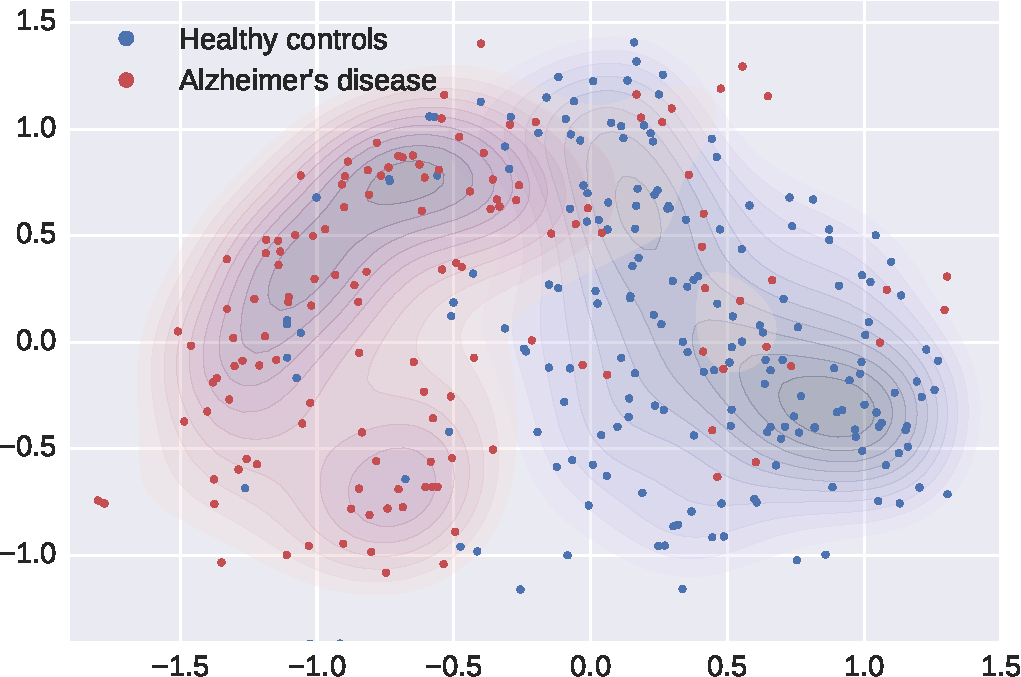
\includegraphics[width=0.8\textwidth]{img/dr.pdf}\label{fig:dr}
\caption{Структурные коннектомы для всех представителей классов AD и NC, спроецированные на двумерное пространство. Синий и красный цвета обозначают NC и AD группы соответственно. Точки соответствуют графам, прозрачные области отображают оценку плотности ядер для каждой группы}
\end{figure}

Следующая таблица содержит сравнительные результаты классификации всех четырех алгоритмов, рассматривавшихся в работе

\begin{table}[h!]
\centering
\begin{tabular}{lllll}
\hline
\rowcolor[HTML]{EFEFEF} 
Пара классов & SVM + L2 & SVM + SPD & Isomap $\delta_{spsd}$ & SVM + $\delta_{spsd}$ \\
\hline
(AD, NC)     & 77.2 $\pm$ 0.99     & 80 $\pm$ 0.54                           & \cellcolor[HTML]{E1FFCF}81.6 $\pm$ 0.6           & \cellcolor[HTML]{E1FFCF}81.6 $\pm$ 0.7                        \\
(AD, LMCI)   & 65.5 $\pm$ 1.6      & \cellcolor[HTML]{E1FFCF}68.8 $\pm$ 0.81 & 67.8 $\pm$ 0.6                                   & 68.6 $\pm$ 1.4                                                \\
(LMCI, EMCI) & 44.7 $\pm$ 2.9      & \cellcolor[HTML]{E1FFCF}47.8 $\pm$ 2.4  & 34.1 $\pm$ 0.59                                  & 44.1 $\pm$ 2.2                                                \\
(EMCI, NC)   & 50.4 $\pm$ 1.8      & 53.9 $\pm$ 1.6                          & 53.8 $\pm$ 0.12                                  & \cellcolor[HTML]{E1FFCF}{\color[HTML]{000000} 57.1 $\pm$ 1.5}
\end{tabular}
\caption{Сравнительные результаты классификации всех четырех алгоритмов, рассматривавшихся в работе. Цветом выделены лучшие результаты для каждой пары классов. Метрика качества – ROC AUC \eqref{roc-auc}}
\end{table}
\newpage
\indent Из таблицы можно увидеть, что предложенные методы показали себя лучше базовых в задаче классификации пары классов AD vs NC. \\
\indent Более того, метод, основанный на вычислении ядра для SVM c помощью расстояния на многообразии СППО матриц дал значительно лучшие результаты в задаче различения здоровых пациентов и пациентов с ранними когнитивными нарушениями. Это является важным результатом, поскольку задача ранней диагностики развития нейродегенеративных заболеваний крайне важна. % +
\newpage\chapter{Заключение}
\indent В этой работе были рассмотрены различные подходы к классификации нейрологических данных на примере данных электроэнцефалографии, функциональной и структурной магнитно-резонансной томографии. Также был рассмотрен математический аппарат, используемый в алгоритмах для этой задачи, а именно концепции геометрии Римана, геометрия многообразия симметричных положительно определенных (СПО) матриц и геометрия многообразия симметричных положительно полуопределенных (СППО) матриц. Геометрия многообразия СПО матриц хорошо изучена и является сильным инструментом, использовавшимся в большом количестве работ по этой теме. Однако геометрия пространства СППО матриц изучена гораздо меньше и до сих пор не применялясь в практических задачах машинного обучения, в частности в задаче классификации данных МРТ.\\
\indent В первой главе работы был дан обзор задачи, кратко описаны основные подходы и объяснена важность задачи. Во второй главе были разобраны техники неизвазивного исследования головного мозга, а именно функциональная и структурная МРТ, а также введено понятие графа функциональных либо структурных связей мозга – коннектома. В третьей главе был выполнен обзор существующих работ по задаче классификации снимков МРТ и кратко представлены полученные в них результаты. \\
\indent В четвертой главе подробно описан используемый в этой работе математический аппарат: в первой части были введены общие определения и обозначения; во второй части разобрана геометрия Римана на примере многообразия СПО матриц: описано многообразие, существующая на нем метрика, геодезические на многообразии и процесс проецирования на касательное пространство; в третьей части введена теория, описывающая многообразие СППО матриц: описана метрика на этом многообразии, горизонтальное пространство к этому многообразию, разобран процесс построения геодезических кривых между СППО матрицами и задана метрика сходства матриц, условно названная расстоянием. \\
\indent В пятой главе подробно рассмотрены два основных подхода в классификации СПО матриц, а именно, ядерные методы на основе расстояния между СПО матрицами и класификация в касательном пространстве, важным шагом которой является проекция на касательное пространство исходных СПО матриц. В шестой главе предложено два метода решения задачи классификации коннектомов, оба из которых первым шагом имеют конвертацию коннектомов в СППО матрицы с помощью преобразования Лапласа: первый метод основан на снижении размерности данных с помощью алгоритма Isomap и классификации данных с помощью логистической регрессии, второй является принципиально новым подходом, не использовавшимся ранее, и основан на примерении геометрии пространства СППО матриц, описанной в пятой главе, для построения положительно определенного ядра с помощью расстояния между СППО матрицами на изначальном многообразии. \\
\indent В главе семь описаны данные, на которых производились вычисления, и постановка экспериментов. Было рассмотрено два эксперимента: влияние ранга матрицы на точность классификации (для этого было произведено искусственное снижение ранга СППО матриц) и сравнение результатов классификации двух существовавших и двух предложенных методов. В главе восемь произведен анализ результатов, показавших, что предложенные алгоритмы успешно решают задачу классификации снимков здоровых людей и людей с болезнью Альцгеймера. Также важным результатом является то, что предложенный алгоритм на основе расстояния на многообразии СППО матриц показал результаты, значительно превосходящие результаты остальных алгоритмов, в задаче классификации снимков здоровых людей и снимков людей с ранними когнитивными нарушениями, что позволяет решать задачу ранней диагностики нейродегенеративнх заболеваний. % +
\nocite{*}
\newpage\bibliography{ref}{}
\bibliographystyle{apalike}

\addtocounter{totfigures}{\value{figure}}
\addtocounter{tottables}{\value{table}}

\begin{appendices}
\renewcommand\thechapter{\Asbuk{chapter}}
\setcounter{chapter}{0}

\includepdfset{nup=1x2,frame=true,delta=10mm 10mm,noautoscale=true}

\end{appendices}

\end{document}
